\documentclass[12pt]{article}

\usepackage{sbc-template}
\usepackage{graphicx,url}
\usepackage[utf8]{inputenc}
\usepackage[brazil]{babel}
%\usepackage[latin1]{inputenc}  
\usepackage{setspace}
     
\sloppy
\title{Pipeline: Uma Técnica de Programação Paralela}
\vspace{0.5cm}
\author{Erick Modesto Campos}
\vspace{0.5cm}

\address{Instituto de Ciência Exatas e Naturais (ICEN) -- Universidade Federal do Pará
  (UFPA)\\
  Laboratório de Visualização, Interação e Sistemas Inteligentes (LabVis - UFPA)\\
  Cep 66075110 -- Belém -- Pará -- Brazil
  \email{erick.c.modesto@gmail.com / erickcampos@ufpa.br}
}


\begin{document} 

\onehalfspace
\maketitle

\begin{abstract}
   With the evolution of microprocessors, the execution of sequential tasks has
   become increasingly unfeasible to be applied in scenarios where the issue of
   performance must be considered. Therefore, parallel programming techniques
   are essential to extract maximum performance in sequential task tasks.
   Therefore, parallel programming techniques are essential to extract maximum
   performance in serial tasks. In this sense, the so-called pipeline technique
   may be a good alternative for improving performance in applications.

\end{abstract}
     
\begin{resumo}
  Com a evolução dos microprocessadores, a execução de tarefas sequenciais foi
  se tornanando cada vez mais inviável de ser aplicado em cenários onde a
  questão do desempenho deve ser considerado. Por isso, técnicas de programação
  paralela são imprescindíveis para extrair o máximo de desempenho em tarefas
  de tarefas sequenciais. Nesse sentido, a técnica denominada de pipeline pode
  ser uma boa alternativa para a melhora de desenpenho em aplicações.
\end{resumo}

\begin{section}{Introdução}
Em algumas décadas atrás, era difícil prever que os computadores se tornariam
tão populares no cotidiano de bilhões de pessoas. Os primeiros computadores,
como o ENIAC (\textit{Electronic Numerical Integrator and Computer}), por
exemplo, foram desenvolvidos para realizar funções extremamente específicas que
limitavam seu uso. A programação nesses computadores era realizada através de
válvulas mecânicas que assumiam valores binários e precisava de uma grande
quantidade de pessoas para realizar essa tarefa.

Foi com a chegada dos chamados computadores pessoais (PC, do inglês
\textit{personal computer}) que a população começou a ter acesso a essa
tecnologia. O primeiro microcomputador surgiu em 1974, desenvolvido pela empresa
MITS (\textit{Micro Instrumentation Telemetry Systems}), e possuia um
microprocessador de 8 bits operando a 2~MHz que já era capaz de realizar
operações mais variadas, se comparado ao ENIAC, por exemplo, que foi
desenvolvido para ralizar cálculos balísticos.

Conforme os anos foram passando, o poder de processamento dos computadores foram
crescendo significativamente. A Tabela~\ref{tab:cpu} extraída
de~\cite{Evolutio17} mostra a evolução do poder de processamento dos
microprocessadores.

%\vspace{1cm} 
\begin{table}[h!]
\centering
\caption{Evolução dos microprocessadores.}
\label{tab:cpu}
\begin{tabular}{ccccc} % <-- Alignments: 1st column left, 2nd middle and 3rd right, with vertical lines in between
\hline
\textbf{Processador} & \textbf{Ano} & \textbf{Transistores} & \textbf{Dados} & \textbf{Clock}\\
8080 & 1974 & 6.000 & 8 bits & 2~MHz \\
8085 & 1976 & 6.500 & 8 bits & 5~MHz \\
8086 & 1978 & 29.000 & 16 bits & 5~MHz \\
8088 & 1979 & 29.000 & 8 bits & 5~MHz \\
80286 & 1982 & 134.000 & 16 bits & 6~MHz \\
80386 & 1985 & 275.000 & 32 bits & 16~MHz \\ 
80486 & 1989 & 1.200.000 & 32 bits & 25~MHz \\
PENTIUM & 1993 & 3.100.000 & 32/64 bits & 60~MHz \\ 
PENTIUM II & 1997 & 7.500.000 & 64 bits & 233~MHz \\
PENTIUM III & 1999 & 9.500.000 & 64 bits & 450~MHz \\
PENTIUM IV & 2000 & 42.000.000 & 64 bits & 1.5~GHz \\
\hline
\end{tabular}
\end{table}
 %\vspace{1cm} 

Com esse crescente poder computacional dos micropocessadores que possuem
multiplos núcleos, a busca em extrair ao máximo a capacidade de processamento, a
aplicação de técnicas de programação paralela são necessários nesse cenário.
Nesse sentido, a utilização do pipelining é uma boa alternativa para melhorar o
desempenho de tarefas seriais.



\end{section}
\begin{section}{Pipelining}
Esta seção apresenta trabalhos que utilizaram algum tipo de sistema embarcado
para realizar tarefas de processamento digital de imagens. Apesar deste trabalho
utilizar o Raspberry Pi, os trabalhos apresentados a seguir utilizam também
outras palataformas embarcadas. O objetivo desta seção é mostrar os trabalhos
que utilizaram processamento de imagens através de uma abordagem sequencial e
paralela.

\begin{subsection}{Processamento Sequencial}

Técnicas de processamento digital de imagens foram aplicadas no trabalho
desenvolvido em~\cite{Karthik16} para detectar doenças em bananeiras através do
reconhecimento de padrões em imagens de folhas de bananeiras. O algoritmo
alaborado foi executado em uma BeagleBone Black~\cite{beagle}, uma plataforma
embarcado que possui um ARM Cortex-A8 com dois núcleos de processamento. Apesar
de ser \textit{dual core} todas as tarefas do algoritmo foram projetadas para
serem executadas de forma sequential, visto que não era realizado um processamento
em massa, já que bastava uma foto capturada por uma \textit{webcam} no momento 
desejado para que a detecção da imagem fosse concluída.

O trabalho proposto em~\cite{Batista17} utilizou algoritmos sequenciais de
processamento de imagens para realzar o reconhecimento de gestos da cabeça do
usuário e transformá-los em comandos de controle para um televisor. Para isso,
foi utilizados as plataformas embarcadas C.H.I.P.~\cite{chip} e
Arduino~\cite{Arduino}. O C.H.I.P. é uma placa de baixo custo, assim como o
Raspberry Pi, mas que possui um processador \textit{single core} o que
inviabilizou o uso de técnicas de processamento paralelo para o reconhecimento
de gesros da cabeça do usuário. Já o Arduíno, é uma plataforma que possui um
microcontrolador de 8 bits que foi utilizado apenas para o envio de sinais
infravermelho de controle para o televisor a ser controlado. 

Já em~\cite{Li09} foi utilizado um FPGA (do inglês \textit{Field-Programmable
Gate Array}), um dispositivo semicondutor baseado em uma matriz de blocos
lógicos configuráveis (BLC) conectados via interconexões
programáveis~\cite{fpga}, para realzar a tarefa de aquisição e também de
processamento de imagens. O objetivo do trabalho era realizar tarefas de
processamento de imagens utilizando uma plataforma simples e relativamente mais
barata. Os algoritmos foram utilizados de forma sequencial, pois as tarefas 
constistiam basicamente em cálculos matemáticos simples baseados nos espaços 
de cores.  


\end{subsection}



\begin{subsection}{Processamento Paralelo}

O trabalho proposto em~\cite{Sivaranjani15} utilizou algoritmos de processamento de
imagens para extração de características de impressões digitais dos mãos e dos
pés. Para isso, foi utilizado um Raspberry Pi com uma distribuição do Debian
modificada para plataformas embarcadas. O algoritmo necessário para o
reconhecimento de imagens para extração de recursos biométricos é realizado
usando o OpenCV-2.4.9~\cite{opencv} --- uma biblioteca de código aberto multiplataforma
voltado para visão computacional --- usando o CMake, g ++,
Makefile. Para realzar essa detecção, quatro diferentes algoritmos foram
modificados para serem executados de forma paralela com o intuito de aproveitar
ao máximo o poder de processamento da plataforma utilizada.


Em~\cite{Markovic18} foi utilizado um \textit{cluster} contendo dez Raspberry
Pi 2 Modelo B com o intuito de aumentar o poder computacional
para realizar tarefas de processamento de imagens utilizando um processamento
paralelo. Foi aplicado um algoritmo de detecção de bordas de objetos com a
intenção de segmentar a imagem em bordas. O experimento conduzido no trabalho
utilizou três tarefas de segmentação. A primeira tarefa foi segmentar três
imagens, em seguida seis imagens e por fim nove imagens. Cada experimento foi
executado utilizando técnicas de processamento paralelo em apenas um arduíndo e
também no \textit{cluster}. 


\end{subsection}

\end{section}
\begin{section}{Aplicações de Pipelining}
Esta seção tem como objetivo mostrar a metodogia para implementação do trabalho
proposto.

\begin{subsection}{Forma Sequencial Implementada}


\begin{figure}[!h]
	\centering
	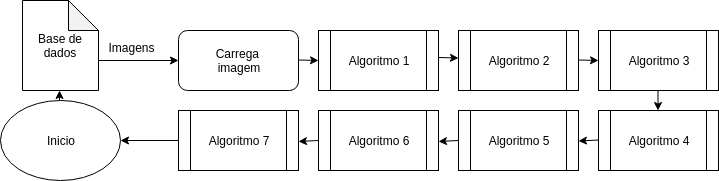
\includegraphics[width=0.95\linewidth]{figs/Sequential.png}
	\caption{Forma sequencial do algoritmo.}
	\label{fig:gray}
\end{figure}



A maioria das imagens digitais é composta por três canais de cores separados: um
canal vermelho, um canal verde e um canal azul. A sobreposição desses canais em
camadas cria uma imagem colorida. Modelos de cores diferentes têm canais
diferentes (às vezes os canais são cores, às vezes são outros valores como
luminosidade ou saturação), mas este trabalho se concentra apenas no RGB.

Todos os algoritmos de conversão do canal RGB para escala de cinza utilizam 
o mesmo processo básico que consistem em três etapas:

\begin{itemize}
\item Obter os valores dos canais vermelho, verde e azul de um \textit{pixel}.
\item Relacionar esses valores para transformar em apenas um valor.
\item Substituir os valores originais de vermelho, verde e azul pelo valor calculado
\end{itemize}


\begin{lstlisting}
for each pixel na imagem{

	vermelho = pixel.Red()
	verde = pixel.Green()
	azul = pizel.Blue()

	Obter_Valor_Cinza = cinza

	pixel.Red = cinza
	pixel.Green = cinza
	pixel.Blue = cinza

}
\end{lstlisting}

Os métodos para obtenção do valor cinza para cada algorimo são apresentados a
seguir.


\begin{figure}[!h]
	\centering
	
\includegraphics[width=0.95\linewidth]{figs/gray.png}
	\caption{Resultado dos algoritmos.}
	\label{fig:gray}
\end{figure}

\subsubsection{Algoritmo 1: Média}
O algoritmo baseado na média é a rotina de conversão mais comum em escala de
cinza e o calculo do valor de cinza é obtido a partir da Equação~\ref{eq:media}.

\begin{equation}
\label{eq:media}
cinza = (vermelho + verde + azul)/3
\end{equation}

Essa fórmula gera um equivalente em escala de cinza razoavelmente boa e sua
simplicidade facilita a implementação e otimização. No entanto, esse método não
deixa de ter falhas --- embora rápida e simples, ela faz um mau trabalho em
representar tons de cinza em relação à maneira como os seres humanos percebem a
luminosidade (brilho).


\subsubsection{Algoritmo 2: Luminância}
Esse segundo algoritmo mostra que a densidade do cone no olho humano não é
uniforme entre as cores. Os seres humanos percebem o verde mais fortemente que o
vermelho e o vermelho mais fortemente que o azul. Isso faz sentido do ponto de
vista da biologia evolucionária --- grande parte do mundo natural aparece em
tons de verde, de modo que os humanos desenvolveram maior sensibilidade à luz
verde.

Como os humanos não percebem todas as cores da mesma forma, o ``método da média'' de
conversão em escala de cinza é impreciso. Em vez de tratar as luzes vermelha,
verde e azul igualmente, uma boa conversão em escala de cinza pondera cada cor
com base na maneira como o olho humano a percebe. Uma fórmula comum em
processadores de imagem (Photoshop, GIMP) é apresentada na
Equação~\ref{eq:luminancia}.


\begin{equation}
\label{eq:luminancia}
cinza = (0.3*vermelho + 0.59*verde + 0.11*azul)/3
\end{equation}

\subsubsection{Algoritmo 3: Luma}

Assim como no algoritmo 2, este método tenta uniformizar a forma como o ser
humano perceber as cores. Para isso, também é utilizada uma média ponderada
entre os canais como é mostrado na Equação~\ref{eq:luma}

\begin{equation}
\label{eq:luma}
cinza = (0.2126*vermelho + 0.7152*verde + 0.0722*azul)/3
\end{equation}


\subsubsection{Algoritmo 4: Dessaturação}

A maioria dos programadores usa o modelo de cores RGB. Embora seja uma boa
maneira de uma máquina descrever cores, o espaço de cores RGB pode ser difícil
para a percepção humana. Nesse sentido, o espaço de color HSL (do inglês
\textit{hue, saturation, lightness}) é algumas vezes utilizado para a
vizualização das cores. A matiz (\textit{Hue}) pode ser considerada o nome da
cor --- vermelho, verde, laranja, amarelo etc.  A saturação
(\textit{saturation}) descreve como uma cor é vívida; uma cor muito vívida tem
saturação total, enquanto o cinza não tem saturação. 

A dessaturação de uma imagem funciona convertendo o espaço RGB no espaço HSL e 
forçando a saturação para zero. Um pixel pode ser dessaturado encontrando o
ponto médio entre o máximo de (R, G, B) e o mínimo de (R, G, B), como mostra a
Equação~\ref{eq:dessatura}.

\begin{equation}
\label{eq:dessatura}
cinza = ( Max(vermelho, verde, azul) + Min(vermelho, verde, azul) ) / 2
\end{equation}



\subsubsection{Algoritmo 5: Decomposição}
A decomposição de uma imagem oPde ser considerada uma forma mais simples de
dessaturação. Para decompor uma imagem, cada \textit{pixel} é forçado parao
valor mais alto (máximo) ou mais baixo (mínimo) de seus valores em vermelho,
verde e azul. As Equações~\ref{eq:a} e~\ref{eq:b} mostram como calcular a
decomposição máxima e mínima, respectivamente.

\begin{subequations}

\begin{equation}
\label{eq:a}
cinza = Max(vermelho, verde, azul) 
\end{equation}

\vspace{-1cm}

\begin{equation}
\label{eq:b}
cinza =  Min(vermelho, verde, azul) 
\end{equation}
\end{subequations}


\subsubsection{Algoritmo 6: Canal de cor única}

Este algoritmo representa o método computacional mais simples para conversão em
escala de cinza. Ao contrário de todos os métodos apresentados, este método 
não requer cálculos. Apenas é necessário escolher o valor de um determinado
canal e aplicar para ao valor de cinza, como mostrado na
Equação~\ref{eq:a1},~\ref{eq:b1} e~\ref{eq:c1}

\begin{subequations}

\begin{equation}
\label{eq:a1}
cinza = vermelho 
\end{equation}

\vspace{-1cm}

\begin{equation}
\label{eq:b1}
cinza =  verde 
\end{equation}

\vspace{-1cm}

\begin{equation}
\label{eq:c1}
cinza =  azul 
\end{equation}
\end{subequations}
  
\subsubsection{Algoritmo 7: Tons de cinza}
Este método permite ao usuário especificar quantos tons de cinza a imagem
resultante utilizará. O algoritmo definir o número de tons de cinza da imagem
convertida. Esse método é um pouco mais trabalhoso se comparado com os demais
algoritmos apresentados. Os procedimentos do algoritmo é mostrado a seguir.


\begin{lstlisting}
for each pixel na imagem{
	fator = 255 / (TonsDeCinza - 1)
	metodo = (vermelho + verde + azul)/3
	cinza = (int)((medio / fator) + 0.5) * fator

	//TonsDeCinza: valor entre 2 e 256
}
\end{lstlisting}

\end{subsection}






\end{section}
\begin{section}{Conclusão}
Como descrito, a técnica denominada de pipeline é bastante simples e robusta que
pode ser utilizada em aplicações que demandem melhoria de desempenho na execução
dos processosi. A questão do balanceamneto sempre deve ser levada em
consideração para que o aplicação dessa técnica seja eficaz, contudo nem sempre
é fácil balancear as subtarefas. Portanto, se uma aplicação necessitar ser
executada com um desempenho superior às tarefas seriais, o pipelining pode ser
uma boa alternativa a ser aplicada nesse caso.


\end{section}
\newpage
\bibliographystyle{sbc}
\bibliography{sbc-template}

\end{document}
